\documentclass[t]{beamer} %% alles am TOP ausrichten, c=CENTER ist default.
%% \documentclass[pausesections]{beamer}
% \documentclass[handout]{beamer}

% \usepackage{pgfpages}
%% \pgfpagesuselayout{4 on 1}[a4paper, border shrink 5mm]
% \pgfpagesuselayout{2 on 1}[a4paper, border shrink 5mm]
%% \pgfpagesuselayout{4 on 1}[a4paper, landscape]

\usepackage[latin1]{inputenc}
% \usepackage{times}
\usepackage[T1]{fontenc}
\usepackage{graphicx}
\usepackage{amscd}
\usepackage{mathabx}

\setlength{\parskip}{2mm}

% % don't show title and author in the footer
% \beamertemplatefootempty
% % Navigationssymbole ausblenden:
% \setbeamertemplate{navigation symbols}{}
% % \setbeamertemplate{footline}{}
% %% ohne Navigation:
\beamertemplatenavigationsymbolsempty  

% don't show structure in header
% \beamertemplateheadempty
% fix block title font for acroread
% \setbeamerfont*{block title}{}

\mode<presentation>
{
  % \usetheme{Madrid} %ohne navigation
  % \usetheme{Warsaw}  
  % \usetheme{Hannover} 
  \usetheme{PaloAlto} 
  \setbeamercovered{transparent}
}


\title{  Active strategies for object discovery } 
\author[]{Phil Bradfield, Jan Fabian Schmid}
\date[]{} 
\institute[UHH] {Computer Vision Project\\ Winter 2016}

\subject{Slides}

\pgfdeclareimage[height=1.5cm]{university-logo}{src/UHH-Logo-cut}
\logo{\pgfuseimage{university-logo}}

\begin{document}

%%%%%%%%%%%%%%%%%%%%%%%%%%%%%%%%%%%%%%%%%%%%%%%%%%%%%% 
\begin{frame}
  \titlepage
\end{frame}

\section{Introduction}

\begin{frame}
	\frametitle{ Introduction }
	\begin{block}{The Task}    
		Develop an autonomous mobile system that performs object discovery in its environment.
	\end{block}
	\begin{itemize}
		\item<1-> Find all objects without pre-knowledge
		% The task of finding all objects in a scene without previous knowledge
		% about the scene and the objects is still a largely unsolved problem
		\item<2-> We are not restricted to using only single images
		% Instead, we are able to move the robot to obtain different views on the same scene.
		\begin{itemize}
			\item Application in real environments possible
			\item Additional difficulties to traditional object discovery
		\end{itemize}
		\item<3-> Combine the data of multiple views
		\begin{itemize}
			\item \textbf{S}imultaneous \textbf{L}ocalization \textbf{A}nd \textbf{M}apping (SLAM)
		\end{itemize}
		%Knowing the corresponding robot pose to the views allows to calculate the relative locations of data points from different views, which can be used to form a map
		\item<4-> Find the \textbf{N}ext \textbf{B}est \textbf{V}iew (NBV)
		\begin{itemize}
			\item Problem of active sensing
		\end{itemize}
		% describes a pose that is near and accessible for the robot and promises high information gain
	\end{itemize}
\end{frame}

%\subsection{Application Scenario}
\begin{frame}
	\frametitle{ Application Scenario }
	\begin{columns}
		\begin{column}{0.65\textwidth}
			\begin{itemize}
				\item Table with a set of objects on it
				\begin{itemize}
					\item Objects of different sizes, shape and color
					\item Some objects are occluded
				\end{itemize}
				\item Robot can move freely around the table
			\end{itemize}		
		\end{column}
		\begin{column}{0.3\textwidth}
			\begin{figure}[h]
				\vspace{-0.5cm}
				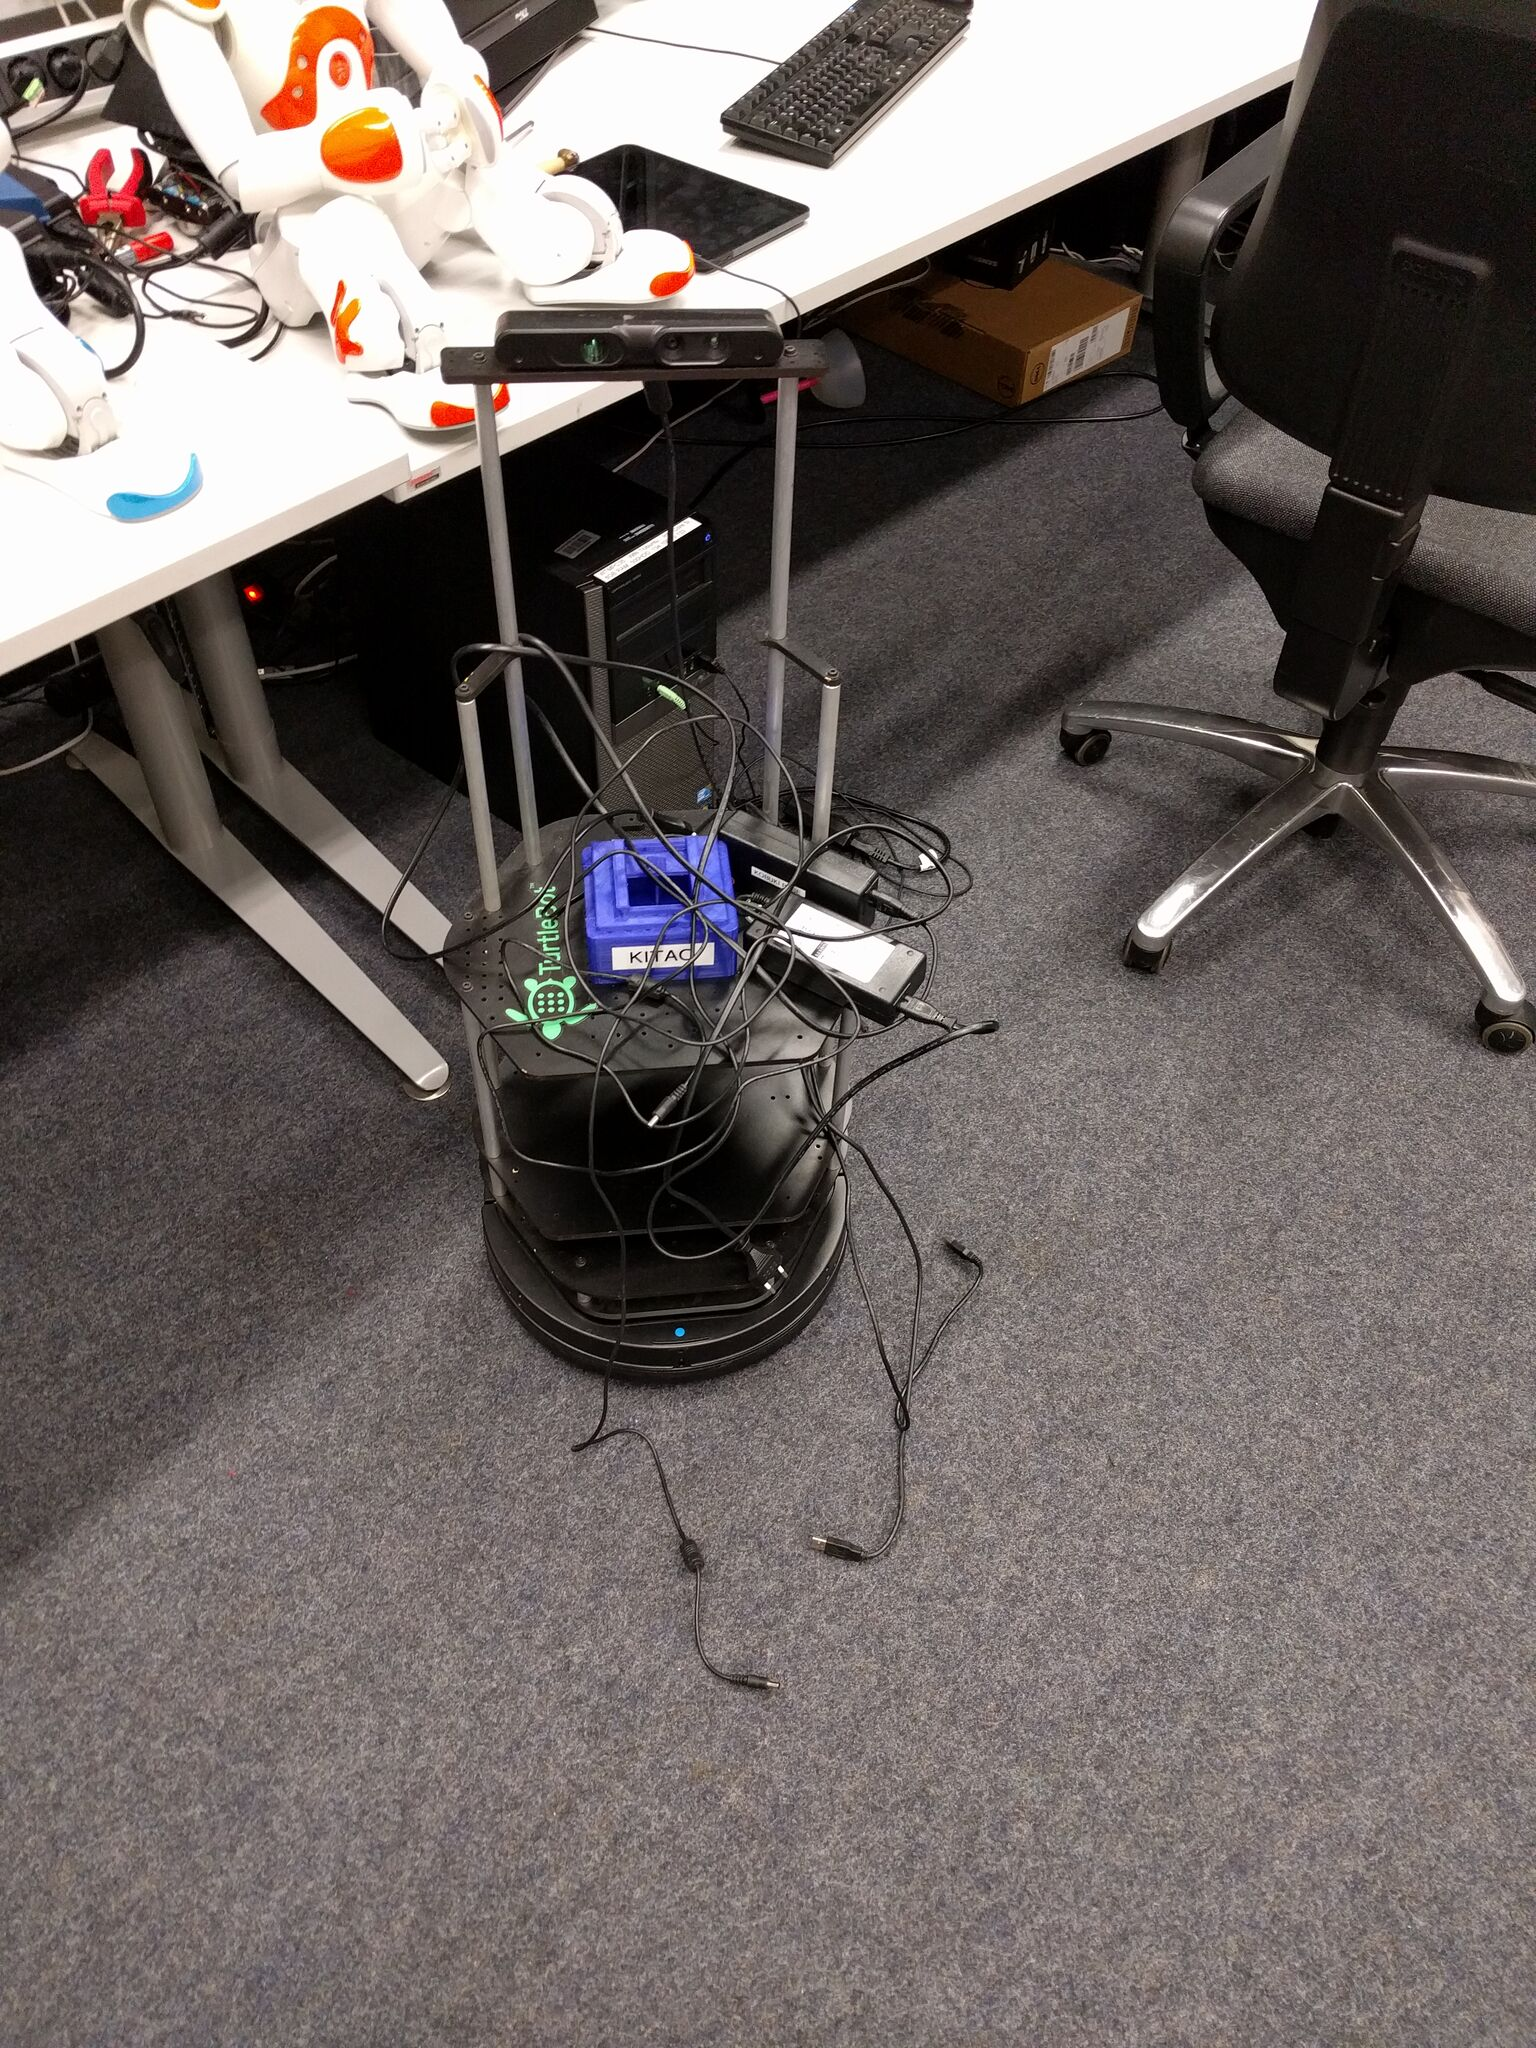
\includegraphics[width=1\textwidth]{src/turtle.jpeg}
			\end{figure}
		\end{column}
	\end{columns}
\end{frame}

%\subsection{Context of mobile systems}
\begin{frame}
	\frametitle{ Context of mobile systems }
	\begin{block}{Limitations}    
		\begin{itemize}
			\item Limited computational processing power
			\item Limited energy
			\item Limited time
		\end{itemize}
	\end{block}
	\begin{itemize}
		\item Focus on relevant aspects of the data
		\begin{itemize}
			\item Next \textbf{best} view is not available
			% The optimal solution to the NBV problem is most likely not available for		applications in real environments, therefore we can only compute approximations. For the very best approximations it might be necessary to consider huge amounts of data.
			\item Don't process every image
			% We will probably use the input from the depth stream in every (or most) timestep to update our 3D map. However, object detection will only be initiated at our desired viewpoints
		\end{itemize}		
		\item Find termination criteria
		% at which point no further investigation of the scene should be performed. Therefore we could find a way to weigh up the energy cost for an operation against the possible benefit that it might provide to solve the task. If there is no operation available for which the information gain is more valuable than the energy then the process stops.
	\end{itemize}
\end{frame}

\subsection{Related Work}
\begin{frame}
	\frametitle{ Related Work - 3D Object Detection }
	\begin{figure}[h]
		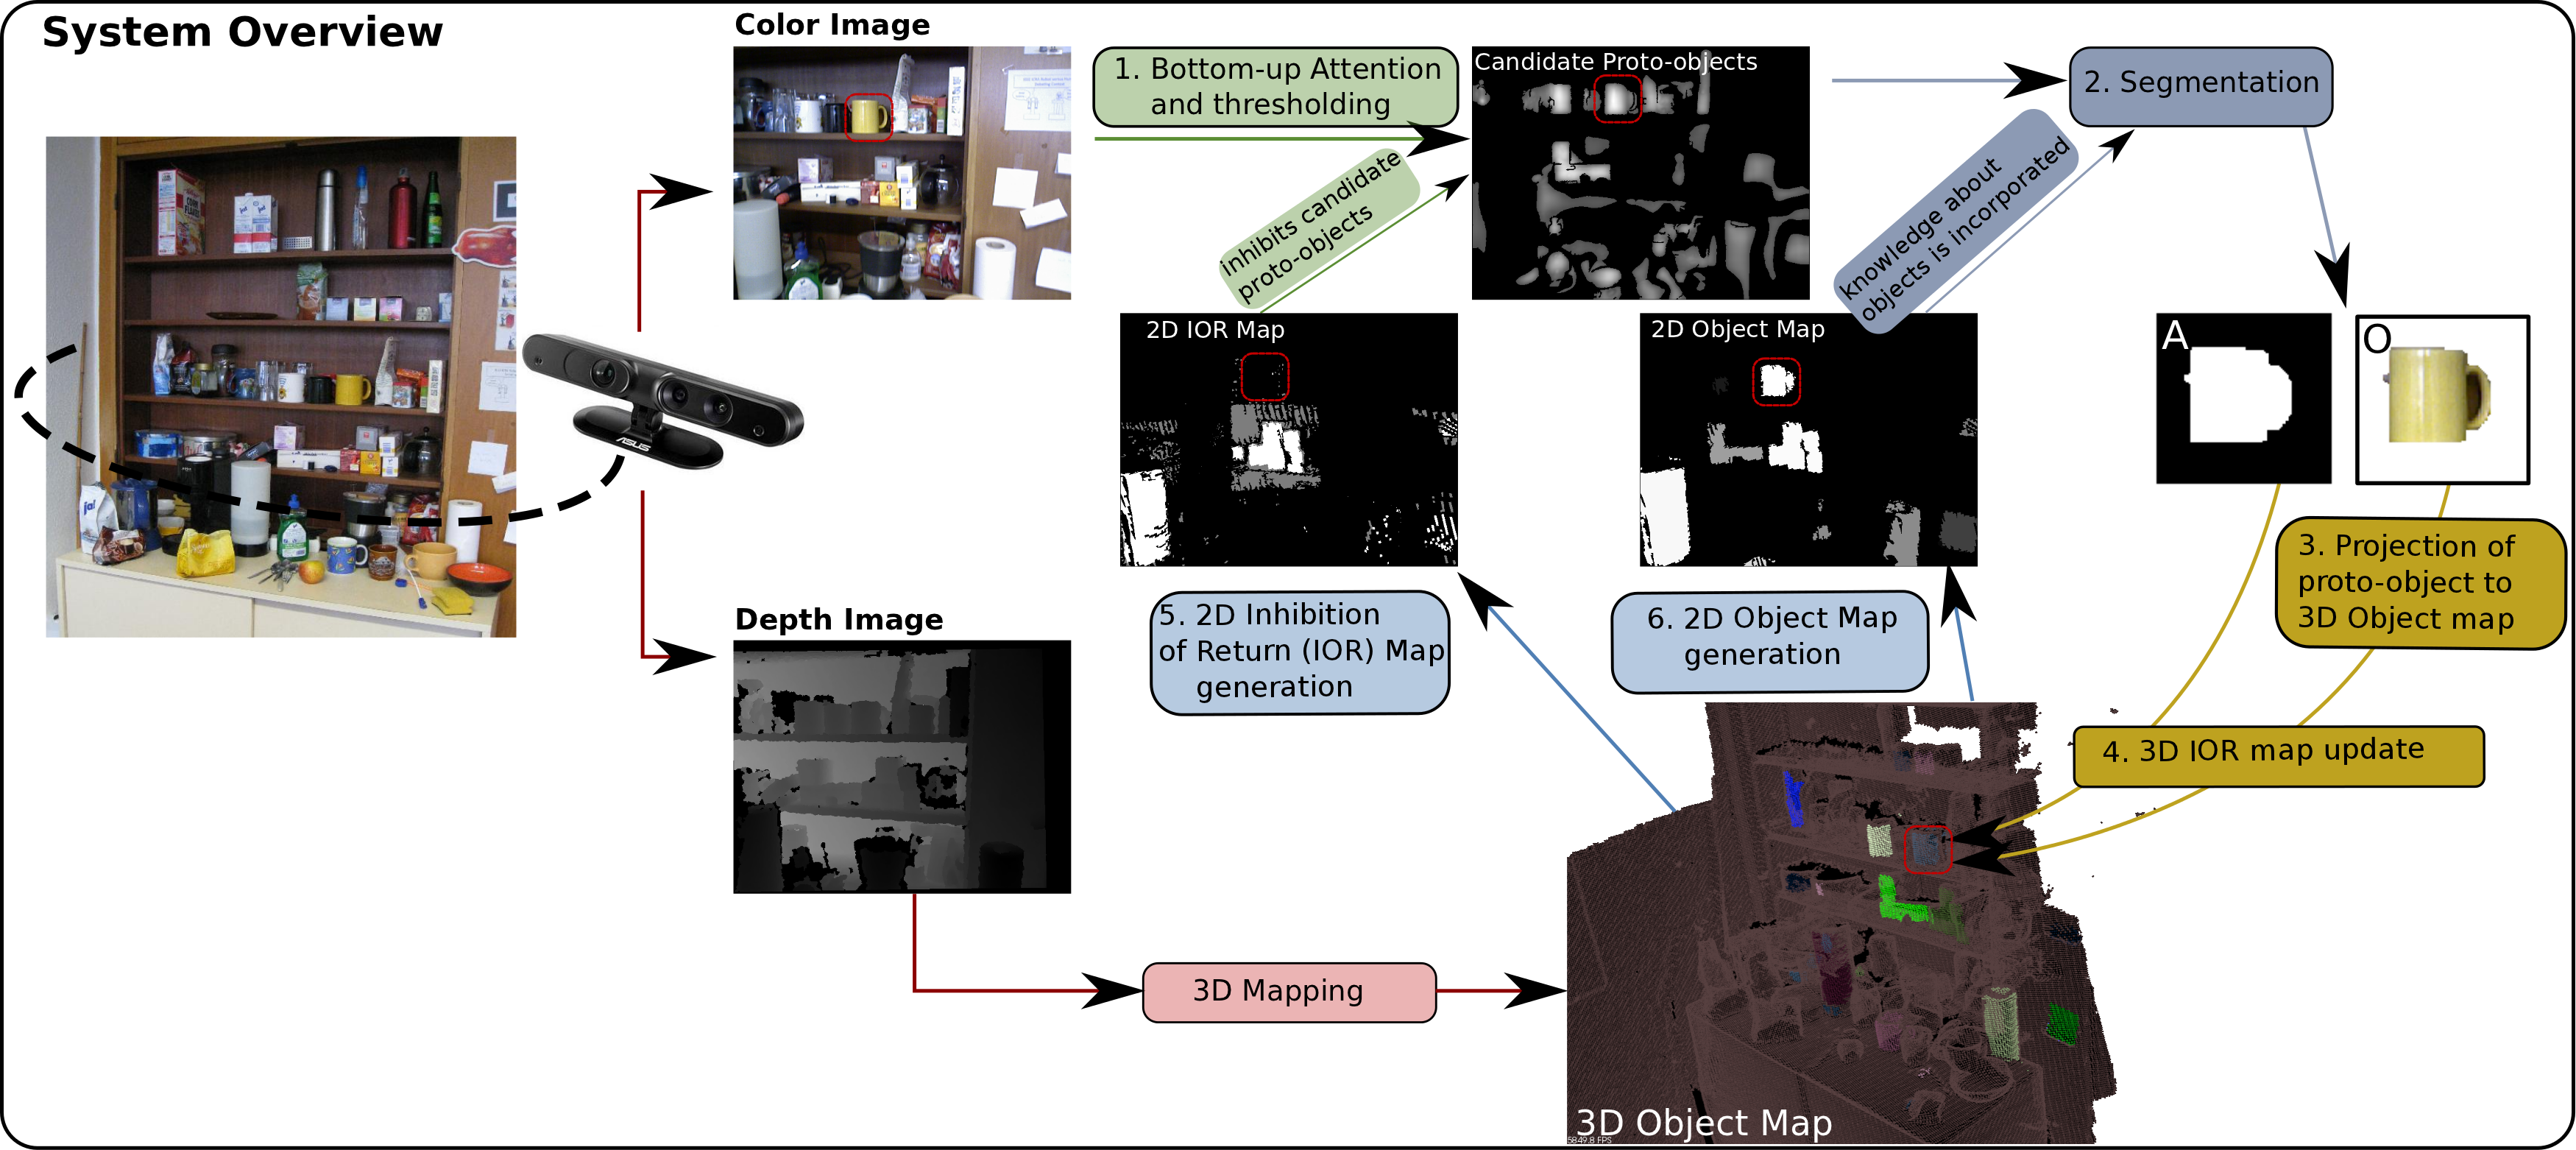
\includegraphics[width=1\textwidth]{src/frintrop.png}
	\end{figure}
	\centering
	\scriptsize [Garc�a and Frintrop, 2013]
\end{frame}

\begin{frame}
	\frametitle{ Related Work - Next Best View}
	\begin{figure}[h]
		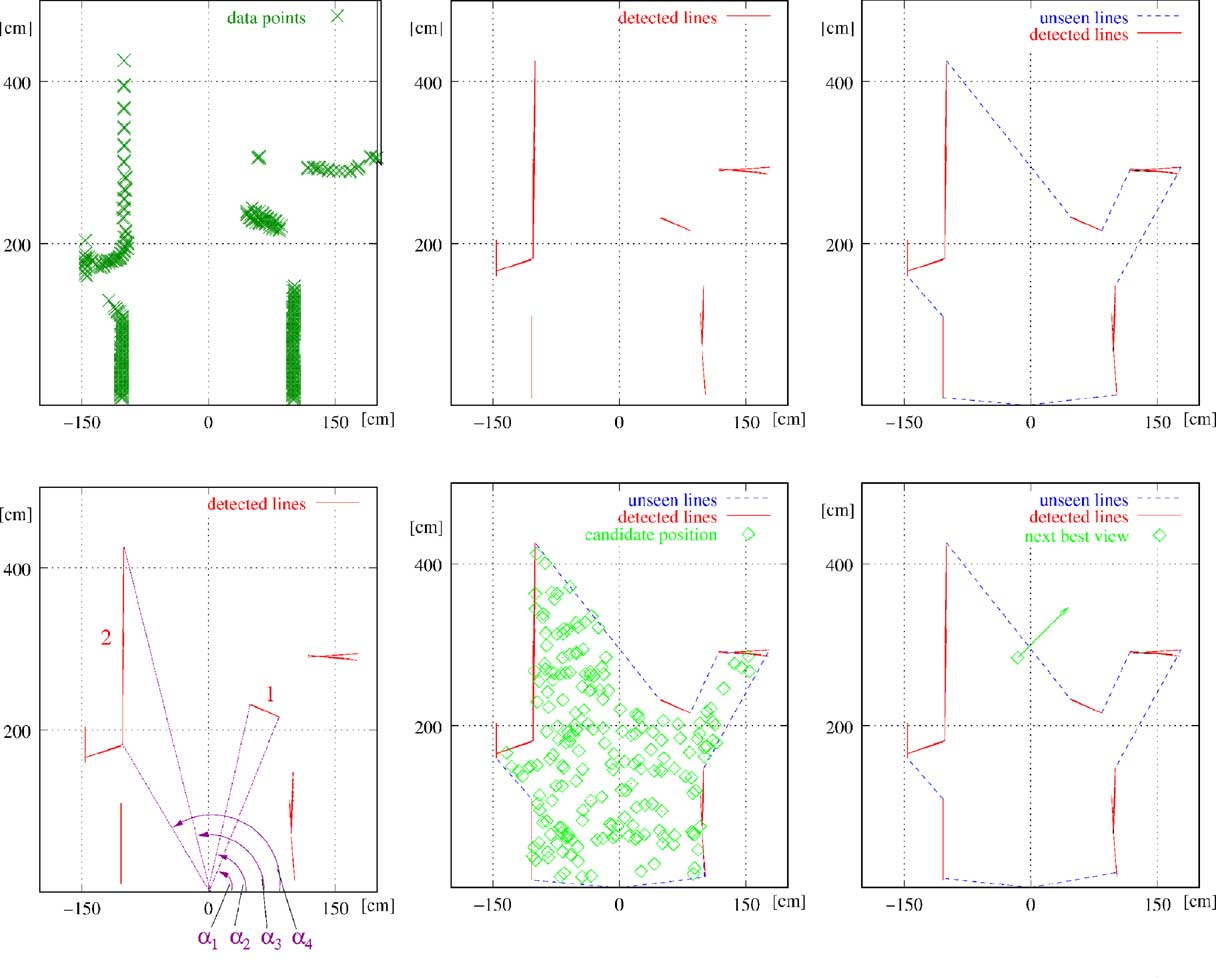
\includegraphics[width=0.8\textwidth]{src/nbv.png}
	\end{figure}
	\centering
	\scriptsize [Surmann et al., 2003]
\end{frame}

\section{Working Plan}
\begin{frame}
	test
\end{frame}

\section{Materials}
\begin{frame}
	test
\end{frame}

\section{Final Output}
\begin{frame}
	test
\end{frame}

\section*{} 
\begin{frame}
	\frametitle{ End of presentation }
	\vspace{1.5cm}
	\textbf{Thank you for your attention!}
\end{frame}

\begin{frame}
	\frametitle{ References }
	\begin{itemize}
		\item Germ�n Mart�n Garc�a and Simone Frintrop. A computational framework for attentional 3d object detection. In Proc. of the Annual Conf. of the Cognitive Science Society. Citeseer, 2013.	
		\item Hartmut Surmann, Andreas N�chter, and Joachim Hertzberg. An autonomous mobile robot with a 3d laser range finder for 3d exploration and digitalization of indoor environments. Robotics and Autonomous Systems, 45(3):181-198, 2003.	
	\end{itemize} 
\end{frame}

\end{document}
